%!TEX program = xelatex
% Note: this template must be compiled with XeLaTeX rather than PDFLaTeX
% due to the custom fonts used. The line above should ensure this happens
% automatically, but if it doesn't, your LaTeX editor should have a simple toggle
% to switch to using XeLaTeX.

\documentclass[
  aspectratio=169, % Uncomment to use an aspect ratio of 16:9 (160 mm by 90 mm)
  %aspectratio=43, % Uncomment to use an aspect ratio of 4:3 (128mm by 96mm)
  t, % Top align all slide content by default
  onlytextwidth, % Typeset content in columns at text width
  10pt, % Default font size, use 10pt for the 16:9 aspect ratio and 8pt for the 4:3 aspect ratio
]{beamer}

\usepackage{../../ImperialTheme/beamer/beamerthemeImperial} % Use the Imperial theme

\def\imagefolder{../../ImperialTheme/beamer/Images}
\def\Rey{\text{Re}}
\title{Finishing incNS - jeff update} % Presentation title to appear on the title slide and left footers

\subtitle{} % Presentation subtitle to appear on the title slide

\author{Víctor Ballester} % Author name(s) to appear on the title slide

\date{\today} % Presentation date to appear on the title slide and right footers

\begin{document}

\begingroup
\setbeamercolor{background canvas}{bg=ICLLightGrey} % Slide background color
\setbeamercolor{title page title}{fg=ICLBlue} % Title text color
\setbeamercolor{title page subtitle}{fg=ICLBlue} % Subtitle text color
\setbeamercolor{author}{fg=ICLBlue} % Author(s) text color
\setbeamercolor{date}{fg=ICLBlue} % Date text color
\setbeamertemplate{title page}[logo]{\imagefolder/ICL_Logo_Blue.pdf} % Imperial logo color, use 'ICL_Logo_White.pdf' for white and 'ICL_Logo_Blue.pdf' for blue
\frame[plain, s]{\titlepage} % Output the title page with no footer ('plain') and vertically distributed text ('s')
\endgroup

\begin{frame}
	\frametitle{Stability analysis diagram}
	\centering

	\begin{itemize}
		\item Nonlinear stability results
	\end{itemize}

	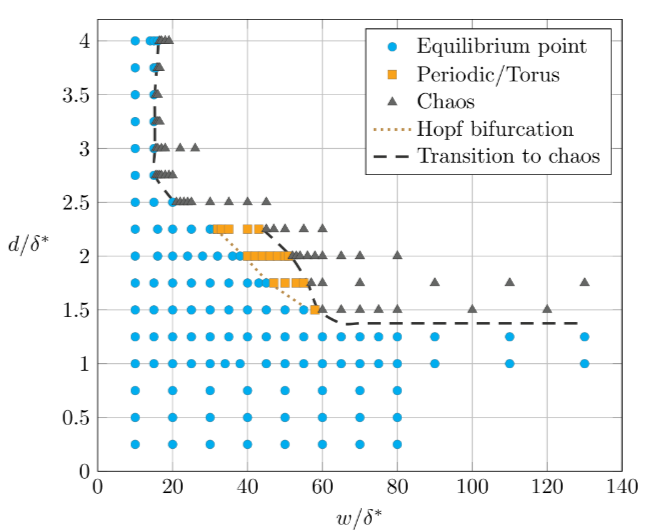
\includegraphics[width=0.5\linewidth]{Images/stabilitycurve.png}
\end{frame}
\begin{frame}
  \frametitle{exciting mechanism}
  \begin{itemize}
    \item To excite the TS modes, we introduce a divergence-free body force to trigger the instability. The force to the streamfunction is defined as
	    $$
	    \psi = A \exp\left(-w[(x-x_0)^2 + (y-y_0)^2]\right) X_t
	    $$

	    where $X_t$ is a white gaussian noise. The point $(x_0,y_0)$ is the location of the forcing and it is located in the BL upstream of the gap.
  \end{itemize}
  
\end{frame}
\begin{frame}
	\frametitle{$\Delta n$-factors curves}
	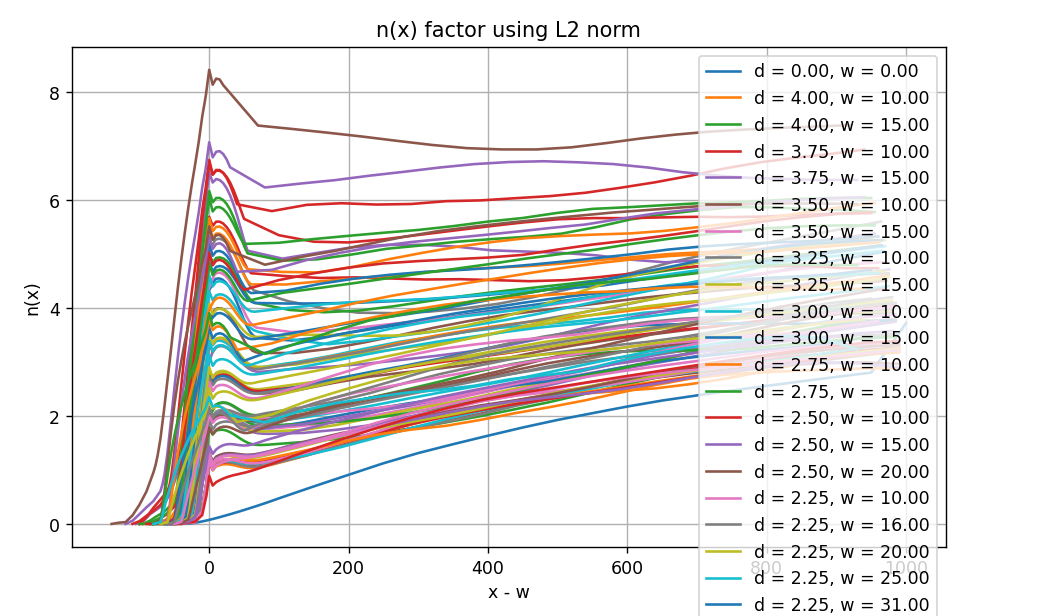
\includegraphics[width=0.8\linewidth]{Images/nfactors.png}
\end{frame}
\begin{frame}
	\frametitle{$\Delta n$-factors}
	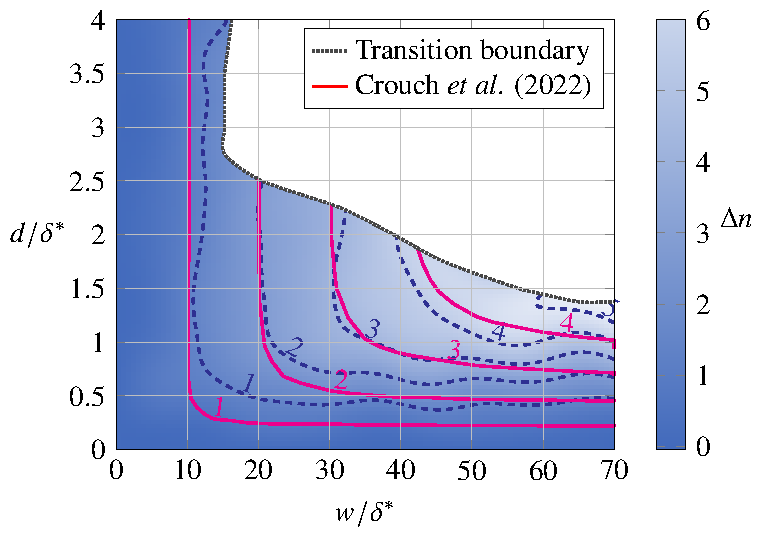
\includegraphics[width=0.7\linewidth]{../../Images/nfactor_countour.pdf}
\end{frame}
\begin{frame}
\begin{columns}[T] % [T] ensures correct vertical alignment
		\begin{column}{0.59\linewidth} % Left column
			\begin{itemize}
			  \item $x_G = 450 mm$
			\end{itemize}
			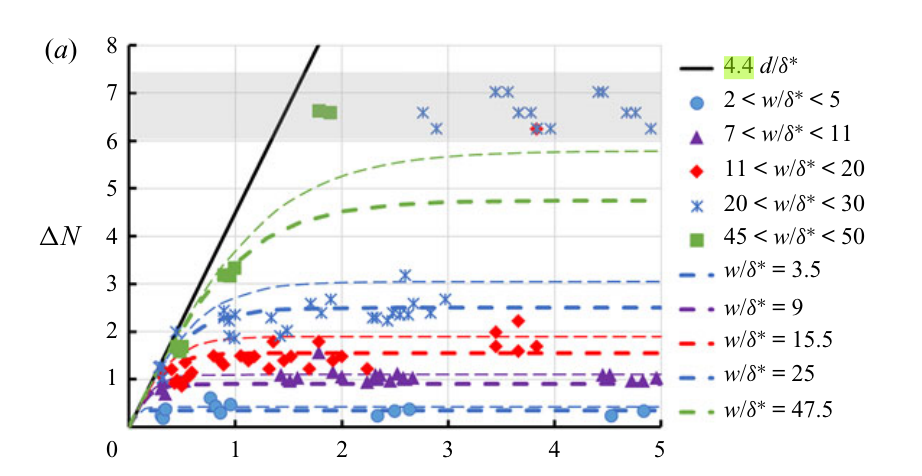
\includegraphics[width=\linewidth]{Images/dvsdN_jeff.png}
			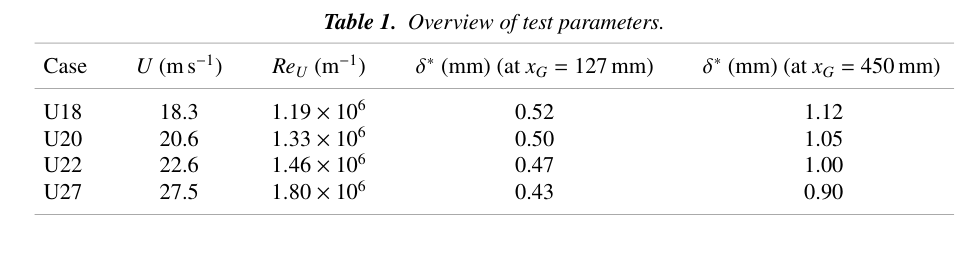
\includegraphics[width=\linewidth]{Images/jeffparam.png}
		\end{column}
		\begin{column}{0.39\linewidth} % Left column
			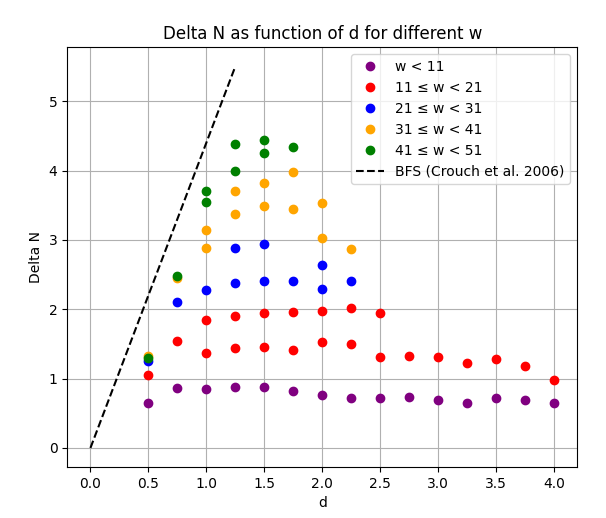
\includegraphics[width=0.98\linewidth]{Images/dvsdN.png}
		\end{column}
	\end{columns}
\end{frame}
\end{document}
